\testfile{pgfplotstest.styles.tex}
\testsection{Style--tests}
\testsubsection{Limits in `every axis'; `cycle list' option and `cycle list name' option}
{
%\tracingmacros=2\tracingcommands=2
\pgfplotsset{every linear axis/.append style={xmin=-3,xmax=3}}
\pgfplotsset{every linear axis/.append style={cycle list name={\blackwhiteplotspeclist}}}
\pgfplotsset{every loglog axis/.append style={cycle list={green\\yellow\\}}}
\begin{tikzpicture}
	\begin{axis}
		\smallplotstest
	\end{axis}
\end{tikzpicture}

\testsubsection{testing `every loglog axis' style}
\begin{tikzpicture}
	\begin{loglogaxis}
		\loglogtestplot
	\end{loglogaxis}
\end{tikzpicture}
}

\testsubsection{Using several `every ...' styles}
{
\pgfplotsset{every axis/.append style={ylabel={$L_2$ Error},line width=1pt,mark=*}}
\pgfplotsset{every axis x label/.append style={name=my x label}}
\pgfplotsset{every axis legend/.append style={legend columns=2}}
\pgfplotsset{every loglog axis/.append style={xmin=1e2,xmax=1e4}}
\begin{tikzpicture}
	\begin{loglogaxis}[xlabel={A -- quite long -- $x$ label}]
	\loglogtestplot
	\end{loglogaxis}
	\fill[red] (my x label.south east) circle(0.3cm);
\end{tikzpicture}
}

\testsubsection{Using the `style=' option}
{
\pgfkeys{/pgfplots/my personal axis/.style={ylabel=Mine!,cycle list name=\blackwhiteplotspeclist,title=My personal title,title style={font=\Huge}}}
\begin{tikzpicture}
	\begin{loglogaxis}[my personal axis]
	\loglogtestplot
	\end{loglogaxis}
\end{tikzpicture}
}

\testsubsection{legend style, grid style, x label style etc. options}
{
\pgfplotsset{every loglog axis/.append style={legend style={legend columns=2,draw=yellow}}}
\pgfplotsset{every axis/.append style={grid style={grid=major}}}
\pgfplotsset{every axis/.append style={x label style={xlabel=Dof,font=\bfseries\Huge},x tick label style={font=\large}}}
\begin{tikzpicture}
	\begin{loglogaxis}
	\loglogtestplot
	\end{loglogaxis}
\end{tikzpicture}

\testsubsection{Providing TikZ-options to either tikzpicture or axis}
\begin{tikzpicture}[color=blue]
	\begin{loglogaxis}
	\loglogtestplot
	\end{loglogaxis}
\end{tikzpicture}

\begin{tikzpicture}
	\begin{loglogaxis}[/tikz/color=blue]
	\loglogtestplot
	\end{loglogaxis}
\end{tikzpicture}
}

\testsubsection{xlabel style and ylabel style}
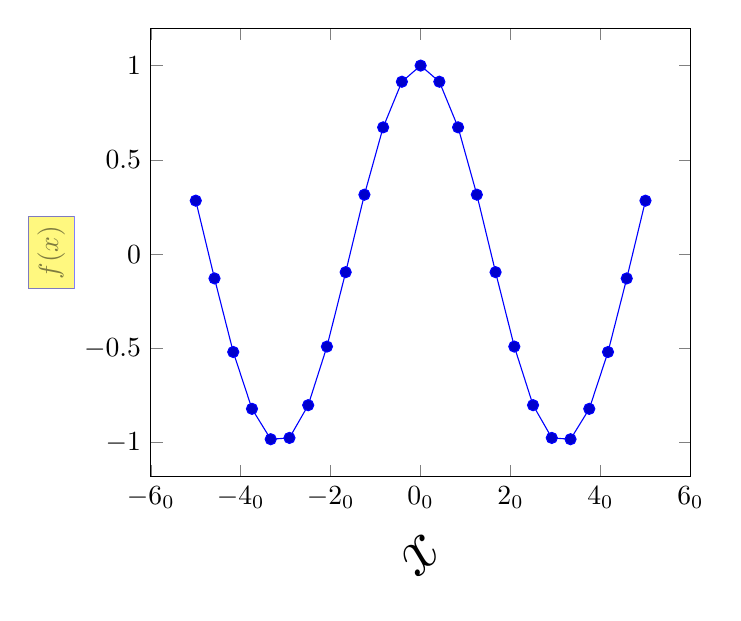
\begin{tikzpicture}
	\begin{axis}[
		xlabel=$x$,
		xlabel style={font=\Huge,rotate=45},
		ylabel=$f(x)$,
		ylabel style={fill=yellow,opacity=0.5},
		y label style={draw=blue},
		xticklabel style={/pgf/number format/.cd,sci,sci subscript},
	]

	\addplot (\x,{cos(\x r)});
	\end{axis}
\end{tikzpicture}

\testsubsection{Collecting many options together}
\begin{tikzpicture}
	\begin{axis}[
		legend style={legend columns=2},
		grid style={draw=brown},
		grid=major,
		max space between ticks=25,
		name=a styled plot,
		y tick label style={/pgf/number format/fixed zerofill,/pgf/number format/use comma,/pgf/number format/precision=3},
		tick label style={/pgf/number format/sci,/pgf/number format/sci e,font=\footnotesize},
	]

	\addplot plot[id=styledplot] function{(40*x**2 - 5*x +3)/2000};
	\addlegendentry{$\frac{1}{2000}(40x^2 - 5x +3)$}
		
	\addplot plot[id=styledplot2] function{(x**5 - 3)/2000};
	\addlegendentry{$\frac{1}{2000}(x^5 - 3)$}
		
	\end{axis}
\end{tikzpicture}

\testsubsubsection{Putting the same options into a style...}
{\pgfkeys{/pgfplots/my style/.style={
		legend style={legend columns=2},
		grid style={draw=brown},
		grid=major,
		max space between ticks=25,
		name=a styled plot,
		y tick label style={/pgf/number format/fixed zerofill,/pgf/number format/use comma,/pgf/number format/precision=3},
		tick label style={/pgf/number format/sci,/pgf/number format/sci e,font=\footnotesize},
		}
}%
\begin{tikzpicture}
	\begin{axis}[my style]

	\addplot plot[id=styledplot] function{(40*x**2 - 5*x +3)/2000};
	\addlegendentry{$\frac{1}{2000}(40x^2 - 5x +3)$}
		
	\addplot plot[id=styledplot2] function{(x**5 - 3)/2000};
	\addlegendentry{$\frac{1}{2000}(x^5 - 3)$}
		
	\end{axis}
\end{tikzpicture}

\testsubsection{Line width}
\testsubsubsection{2pt global}
{
\tikzset{every picture/.style={line width=2pt}}
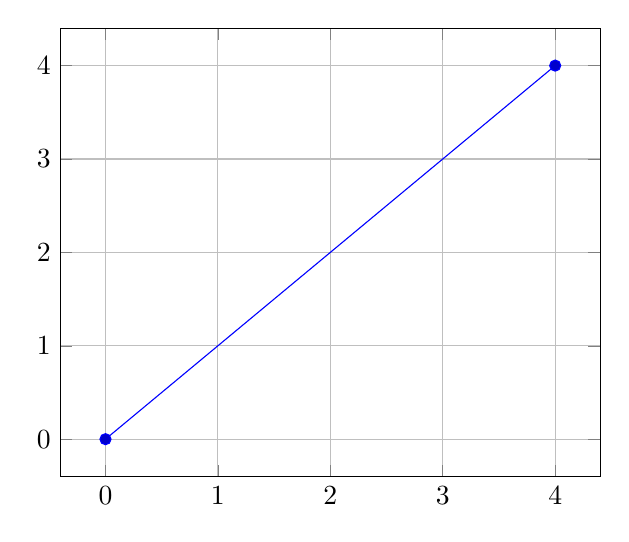
\begin{tikzpicture}
	\begin{axis}[grid =major]
	\addplot coordinates {(0,0) (4,4)};
	\end{axis}
\end{tikzpicture}
}

\testsubsubsection{2pt in every axis}
{
\pgfplotsset{every axis/.append style={line width=2pt}}
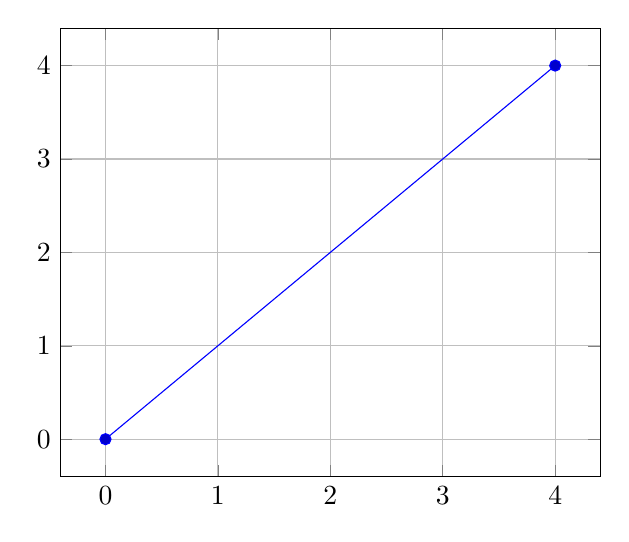
\begin{tikzpicture}
	\begin{axis}[grid =major]
	\addplot coordinates {(0,0) (4,4)};
	\end{axis}
\end{tikzpicture}
}
